\chapter{Foundation}\label{chap:foundation}
\section{Memory Management Unit (MMU)}
\cite{tanenbaum_modern_operating_systems_3}
The memory management unit is a hardware component that manages the
mapping of virtual addresses to physical addresses. The CPU passes
all memory references through the MMU and thus has not to manage the
address translation. This principle can be graphically observed in
figure \ref{fig:tanenbaum_mmu_schematic}.
\begin{figure}
    \centering
    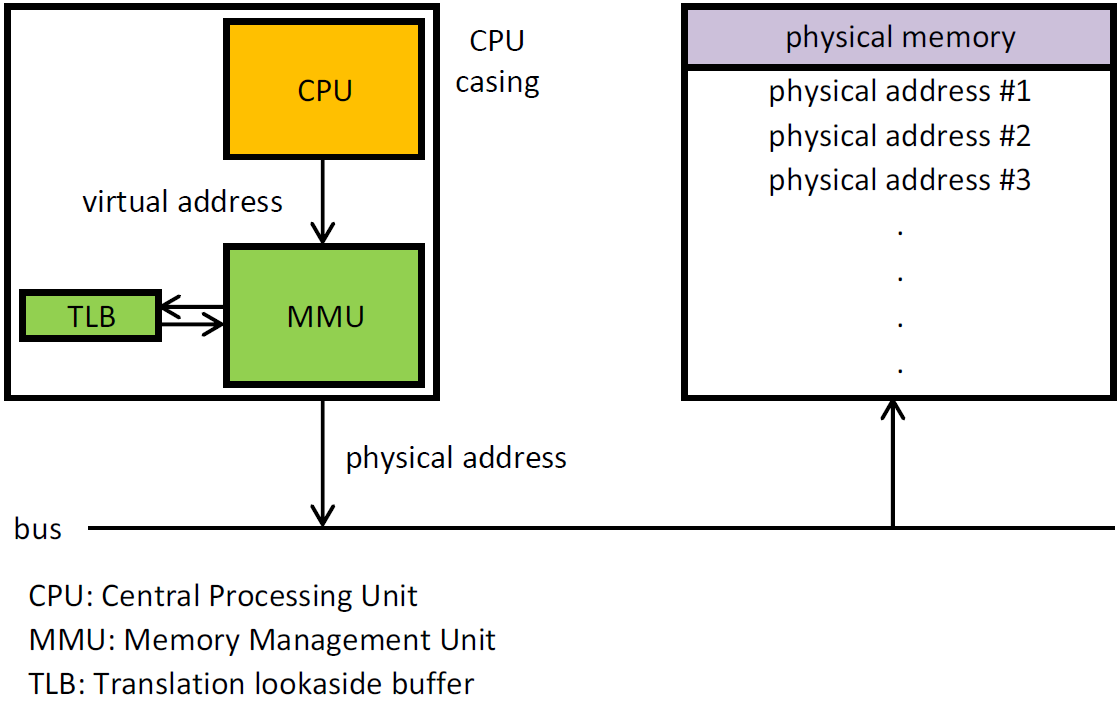
\includegraphics[width=0.5\textwidth]{figures/tanenbaum_MMU_principle_updated}
    \caption{Simplified view on a MMU \cite[p.~186ff]{tanenbaum_modern_operating_systems_3}}
    \label{fig:tanenbaum_mmu_schematic}
\end{figure}
The component is mostly placed directly in the
CPU but can also be a separate integrated chip (mainly old models).
Modern MMUs partition the virtual address space into pages of
size power of 2. As the MMU handles all translations of
page addresses for the CPU, a sufficiently fast translation is important.
To achieve this at least for a limited amount of highly
accessed pages in many implementations a so-called 
translation lookaside buffer (TLB) is used, as can be seen in
figure \ref{fig:tanenbaum_mmu_schematic}.

Most MMU implementations use a so-called \textit{page table} to map
the virtual pages to the physical memory.
One entry of the page table is called \textit{page table entry} and
references the virtual page to a page frame in the physical
memory. Virtual pages can be swapped out to disk if there is
no physical space left. Such \textit{page table entries} do have an
empty reference. If the CPU tries to access such a virtual
page, the MMU notices this access and raises a trap called
page fault. This trap causes the operating system to take
a previously used page frame to be written to the disc
and replace the previous content of this physical memory
space to be replaced with new content.
This principle allows for a nearly unlimited virtual
address space and is especially beneficial for systems
with many concurrent tasks that do not need to run at the
same time.
A representation of a simplified page table can
be seen in figure \ref{fig:tanenbaum_page_table}.
Each page in this example contains 4096 addresses.
\begin{figure}
    \centering
    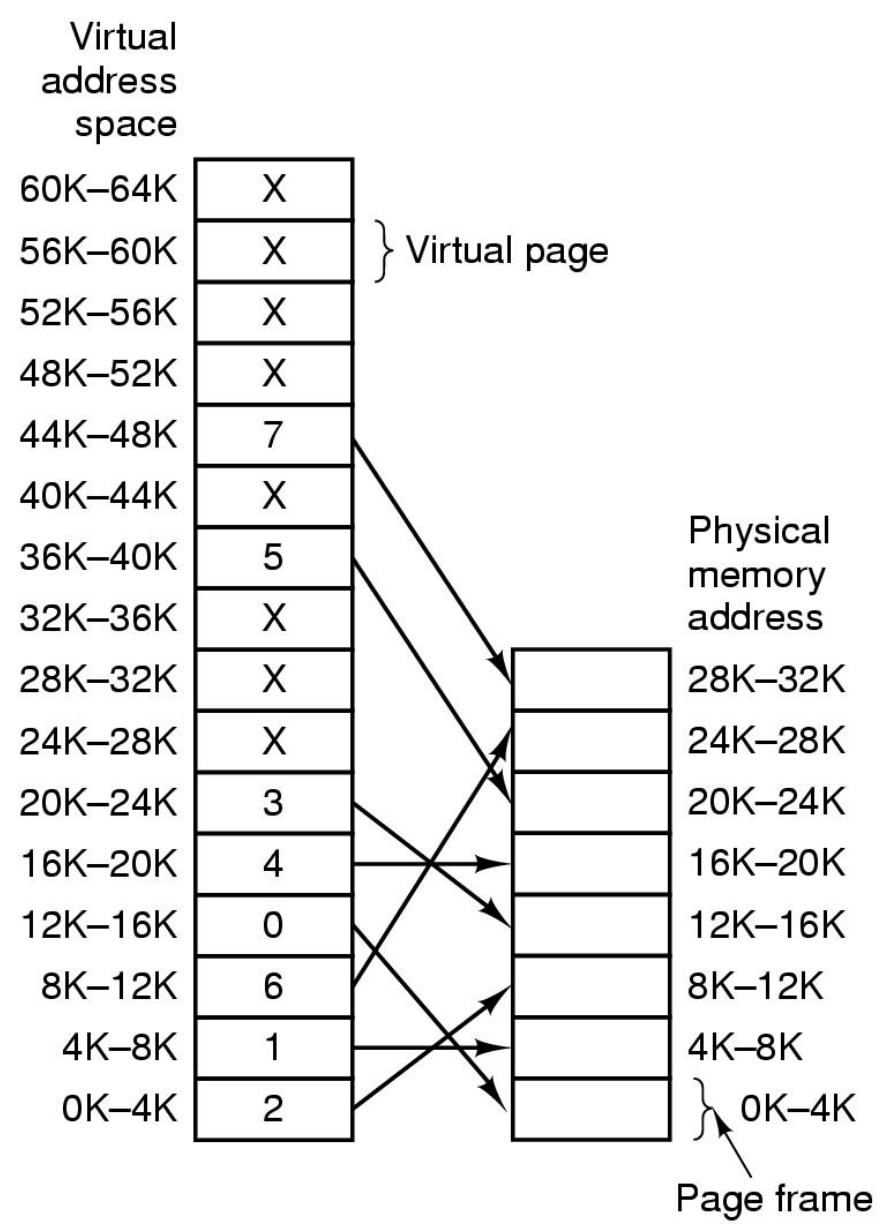
\includegraphics[width=0.5\textwidth]{figures/tanenbaum_page_table}
    \caption{Page table representation \cite[p.~188]{tanenbaum_modern_operating_systems_3}}
    \label{fig:tanenbaum_page_table}
\end{figure}

\section{Checkpoint/Restore Technique}
Checkpoint/Restore \cite{carnegie_checkpoint-restore}, in general, describes the process of 
capturing a certain state of a system and being able
to restore this state at a later stage. 
Checkpointing a system is especially beneficial for processes
that are executed for a long time and are very critical.
In a checkpointed system only the progress since the last
checkpoint is lost.
This technique can mitigate hardware failures and other transient
errors, but there are limits.
Design and programming errors cannot be solved, as the system
returns to the previous state before the crash and
continues the same execution that led to a crash previously.
The system will be stuck in an infinite loop.
Checkpoint/Restore can be used for the whole system or just
parts of it. A good example for the former one is the 
snapshot function of a hypervisor software like
Oracle Virtualbox, QEMU or many other hypervisor programs
which also checkpoint the state of the file system.

\section{FPGA}
To better understand what an FPGA is it will be compared to an ASIC
and a CPU. A Central Processing Unit (CPU) is a very generic
processor and loads its program code from memory.
It is, in its basic form, not optimized for specific tasks
but made for an extensive range of tasks. Parallelization can
only be achieved by adding more CPU cores.
Application-specific integrated circuits (ASICs) are highly
optimized for a minimal scope of predefined tasks.
Algorithms are hardwired and cannot be changed. ASICs
often contain multiple circuits with the same functionality
to speed up the execution. The combination of hard wired
circuits and massive parallel execution make ASICs very
energy efficient. Many processors are paired with an ASIC
to speed up a certain use case. Video acceleration
circuits, for example, can be found in nearly every mobile
processors \cite{arm_gpu_hevc}.

An FPGA is composed out of so-called configurable logic blocks (CLBs)
that performs a certain calculation operation. In figure
\ref{fig:kallstrom_FPGA_cell_example}, an example of a CLB
can be seen. The schematic contains two triple input
Lookup tables (LUTs), a full adder (FA) with a carry in and
carry out signal and a D-type Flip Flop (DFF) 
with a controlling clock signal (clk). The LUTs in this
example define which input (a, b or c) is forwarded to the
FA. Therefore it defines the combinatorial logic of the
computing block.
The FA sums up the two signals plus the carry in signal
it receives and puts out a value plus the carry out signal
for future calculations in other blocks.
As the last step, the DFF reacts to
the clk and sends the result of the
calculation of the FA out.
\begin{figure}
    \centering
    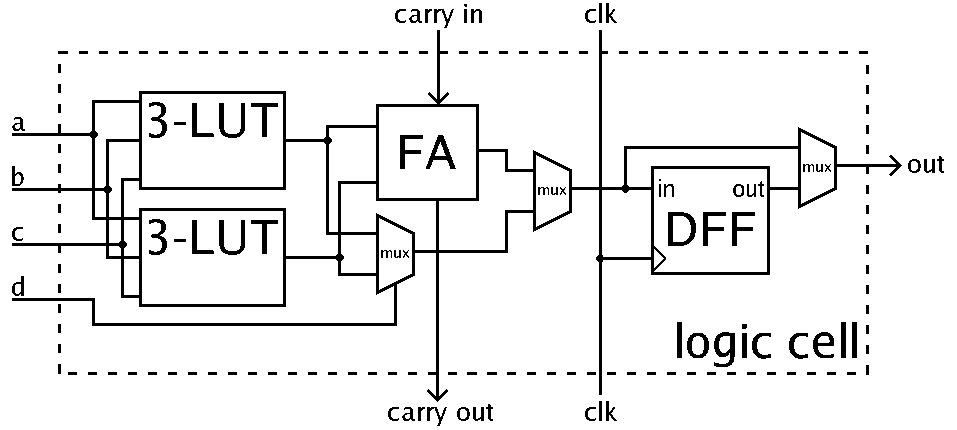
\includegraphics[width=0.8\textwidth]{figures/kallstrom_FPGA_cell_example}
    \caption{Example of a configurable logic block (CLB) \cite{kallstrom_fpga_cell_example}}
    \label{fig:kallstrom_FPGA_cell_example}
\end{figure}
This is one example of a CLB, other implementations
are possible.
To process data, an FPGA needs to group
many CLBs and connect many of them in a meaningful matter.
A simplified schematic of such an FPGA can be seen in
figure \ref{fig:qin_fpga_simplified}.
\begin{figure}
    \centering
    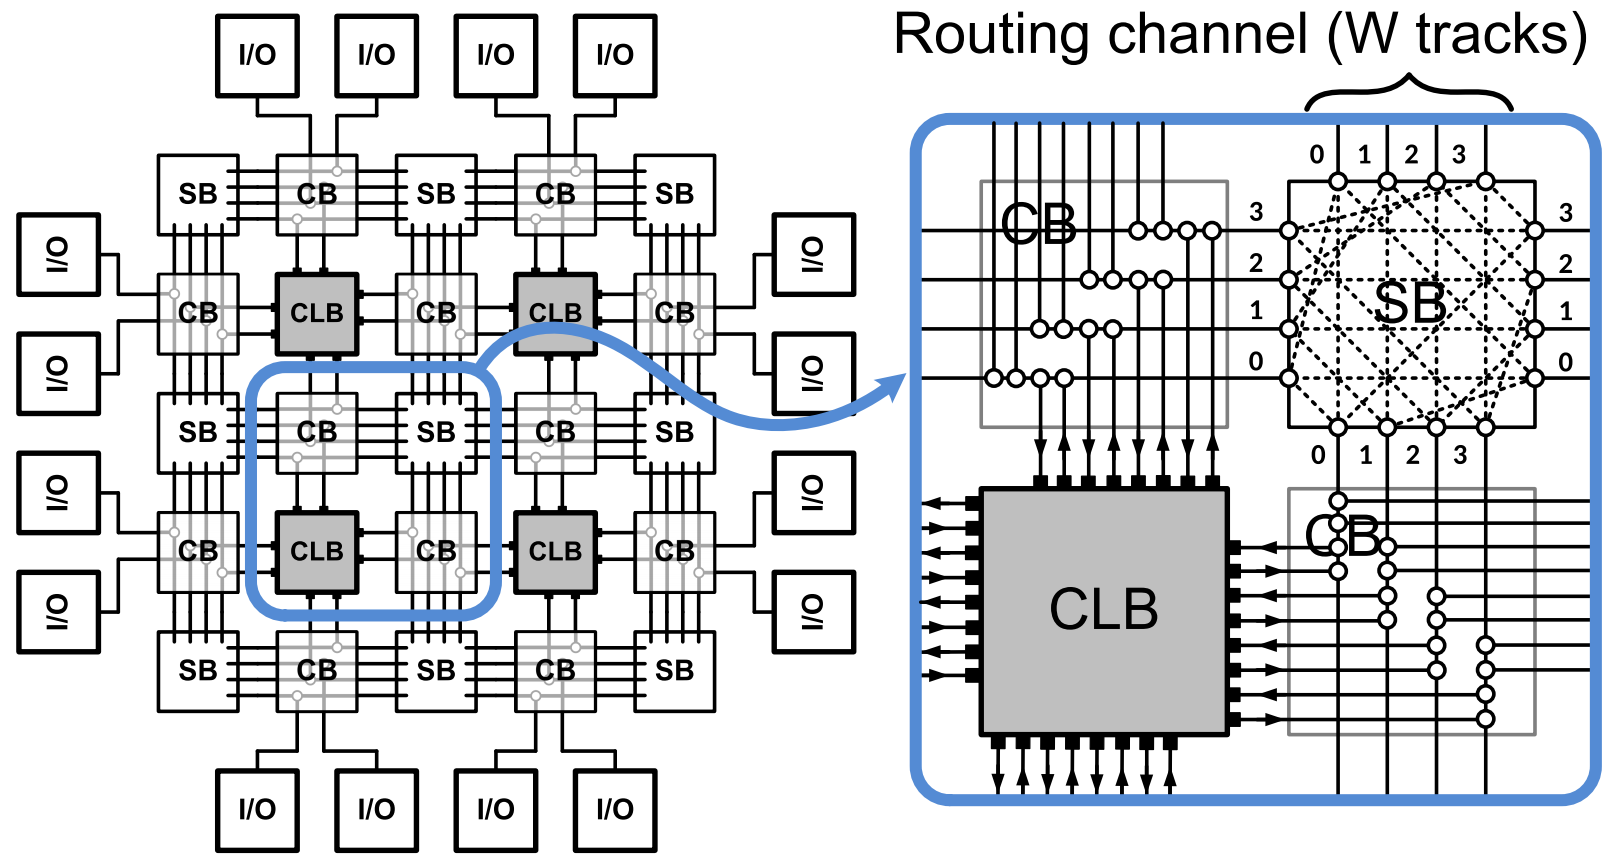
\includegraphics[width=0.8\textwidth]{figures/qin_FPGA_simplified}
    \caption{Simplified FPGA \cite[p.~6]{qin_fpga}}
    \label{fig:qin_fpga_simplified}
\end{figure}
Let us have a look at one of the many quartets of
blocks out of which the core of this FPGA is formed.
One quartet is formed out of one configurable logic block
(CLB) which we already know, two connect boxes (CBs) and
one switch box (SB). The CBs selectively
connect the outputs and inputs of CLBs or SBs to interconnection
channels. The SBs also connect channels
but are more flexible, as they allow horizontal and
vertical connections. At the edges of the FPGA core,
input-output elements (I/Os) can be seen, which are
responsible for inputting and outputting data
into and from the FPGA core.
Other setups are possible. The SBs could, for example,
be exchanged for more CLBs.

When an FPGA is started, no command can be executed
before the instructions for the CLBs, CBs, SBs, and
the I/O elements are loaded from some form of memory
or manually loaded by a programming adapter.
Through this initial step, an internal network is
formed.
